\documentclass[10pt]{exam}
\usepackage[hon]{template-for-exam}
\usepackage{enumitem}
\usepackage{tikz}
\usepackage{multicol,graphicx,cclicenses}
\usetikzlibrary{shadings,decorations.pathmorphing,arrows.meta}



\def\mytitle{Chapter 8 (Rotational Motion)}
\author{Rohrbach}
\date{\today}

\def\mymaketitle{
  \begin{flushleft}
    {\LARGE \textbf \mytitle \par}
  \end{flushleft}
}



\begin{document}


\mymaketitle



\newcommand{\stampbox}[1]{

  \hfill
  \begin{tikzpicture}[every text node part/.style={align=center}]
     \node[gray!50,draw,rounded corners] at (0,0) 
      {\sc Stamp \\ \sc Here \\ \small #1 \sc Points};
  \end{tikzpicture}
  \vspace{1em}
  
  \hrule

}


\begin{center}
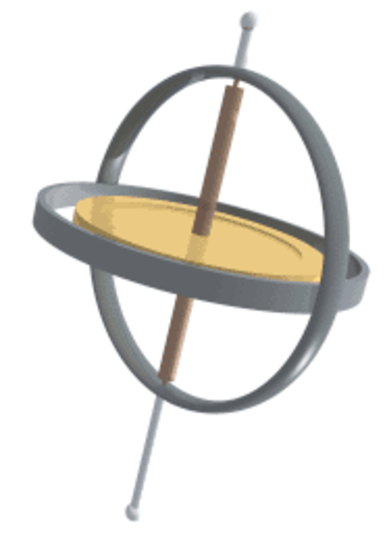
\includegraphics[height=6cm]{gyroscope.pdf}
  
%   {\small``Sketch of a ballistic pendulum before and after it is struck by a bullet'' by \texttt{MikeRun}} 
  
%   \cc\hspace{-1em}\ccby\hspace{-.7em}\ccsa  {\small CC BY-SA 4.0}
  
\end{center}


%%%%%%%%%%%


\section*{Homework Check A (collected XXXXXXXXXX)}


%%%%%%%%%%%


\paragraph{Angular Quantities} p. 222 \#1, 3, 4, 6, 7, 10, 13, 14, 16
\dotfill Complete by Fri, Feb 7

\stampbox{5}

%%%%%%%%%%%



\paragraph{Constant Angular Acceleration \& Rolling} pp. 222-223 \#17, 18, 21, 23
\dotfill Complete by Mon, Feb 10

\hfill \textbf{\emph{Homework Quiz}}

\stampbox{5}


%%%%%%%%%%%


\paragraph{Torque} p. 223 \#24, 26, 27
\dotfill Complete by XXXXXXXXXX

\stampbox{5}



%%%%%%%%%%%




\subsection*{Answers}

\begin{multicols}{3}

  \begin{itemize}[noitemsep]
    \item[1.]  
      (a) $\pi/4~\text{rad} = 0.79~\text{rad} $;  \\
      (b) $\pi/3~\text{rad} = 1.05~\text{rad}$; \\
      (c) $\pi/2~\text{rad} = 1.57~\text{rad}$; \\
      (d) $2\pi~\text{rad} = 6.28~\text{rad}$; \\
      (e) $2.47\pi~\text{rad} = 7.77~\text{rad}$
    \item[3.]  5.32 km
    \item[4.]  $\SI{-170.1}{\radian\per\second^2}$
    \item[6.]  9.2 cm
    \item[7.]  
      $\omega = \SI{230.34}{\radian\per\second}$; \\
      $v = \SI{40.3}{\meter\per\second}$;\\  
      $a = \SI{9280}{\meter\per\second^2}$
    \item[10.]
      $v = \SI{1.9}{\meter\per\second}$;
      $a_C = \SI{3.0}{\meter\per\second^2}$
    \item[13.]  
      $\SI{3500}{\radian\per\second} = 33,000$ rpm
    \item[14.]  
      $\alpha = \SI{4.2}{\radian\per\second^2}$;\\ 
      $a_C = \SI{134}{\meter\per\second^2}$;\\  
      $a_T = \SI{1.3}{\meter\per\second^2}$
    \item[16.]  $\omega_1/\omega_2=R_2/R_1$
    \item[17.]  
      $\SI{-96.3}{\radian\per\second^2}$; 98 rev
    \item[18.]  30,000 rev
    \item[21.]  33.1 m
    \item[23.]  
      \SI{0.533}{\radian\per\second^2}; 12.77 s
    \item[24.]  \SI{86.63}{\meter\newton}
    \item[26.]  
      \SI{40.32}{\meter\newton}; 
      \SI{34.92}{\meter\newton}
    \item[27.]  $l_1 mg-l_2 mg$
  \end{itemize}
  
\end{multicols}

\noindent
{\footnotesize Homework will be accepted for full credit until the test.  Homework turned in after the test will be accepted for half credit until the next test.  \emph{Please remember that you will not be eligible to complete test corrections if you do not turn in your homework.}}

\vspace{1em}



%%%%%%%%%%%%%
%%%%%%%%%%%%%

\pagebreak

\mymaketitle

\section*{Homework Check B (collected on Test Day)}

%%%%%%%%%%%


\paragraph{Rotational Dynamics} pp. 223-225 \#30, 32, 40, 41, 45
\dotfill Complete by XXXXXXXXXX


\stampbox{5}


%%%%%%%%%%%


\paragraph{Rotational KE} p. 225 \#50, 52
\dotfill Complete by XXXXXXXXXX

\stampbox{5}


%%%%%%%%%%%


\paragraph{Angular Momentum} pp. 225-226 \#62, 63, 64, 65
\dotfill Complete by XXXXXXXXXX

\stampbox{5}


%%%%%%%%%%%


\paragraph{Conceptual Questions} p. 220 \#1, 2, 3, 9, 10, 11, 12, 13, 16, 19, 20
\dotfill Complete by XXXXXXXXXX
   
{\sc These questions should have at least one full sentence 
      of explanation}

\stampbox{5}

%%%%%%%%%%%%%%

\paragraph{Misconceptual Questions} p. 191 \#1-13
\dotfill Complete by test day!
   
{\sc You do not need to get this one stamped,
but these are good review for your test!}

\vspace{1em}
\hrule

%%%%%%%%%%%%%%

\paragraph{Bonus Problems!} \#28, 36, 67, 72
\dotfill Turn in separately on test day!

\vspace{1em}
\hrule


%%%%%%%%%%%%%%

\paragraph{Test will be on XXXXXXXXXX} \hfill

\vspace{1em}

\hrule

\subsection*{Problem Answers}

\begin{multicols}{3}

  \begin{itemize}[noitemsep]
    \item[30.]  \SI{1.81}{\kilo\gram \meter^2}
    \item[32.]  \SI{15190}{\meter\newton}
    \item[40.]  
      \SI{-0.0675}{\meter\newton}; \SI{16.38}{\second}
    \item[41.]  
      \SI{324}{\meter\newton}; \SI{129.6}{\newton}
    \item[45.]  31.3 N
    \item[50.]  13,640 J
    \item[52.]  48.8 J
    \item[62.]  1.5
    \item[63.]  $\omega/2$
    \item[64.]  0.38 rot/s
    \item[65.]  \SI{1.23}{\kilo\gram\meter^2}
  \end{itemize}
  
\end{multicols}

\subsection*{Misconceptual Answers}

\begin{multicols}{5}

  \begin{itemize}[noitemsep]
    \item[1.]  C
    \item[2.]  B
    \item[3.]  B
    \item[4.]  C
    \item[5.]  C, E, \& F
    \item[6.]  B
    \item[7.]  B
    \item[8.]  B
    \item[9.]  B
    \item[10.]  A
    \item[11.]  C
    \item[12.]  A
    \item[13.]  A
  \end{itemize}
  
\end{multicols}


\end{document}